% ============================ 三、技术方案 ============================
\section{技术方案：机制受限的双轨系统}
\label{sec:method}

\begin{figure}[H]
\centering
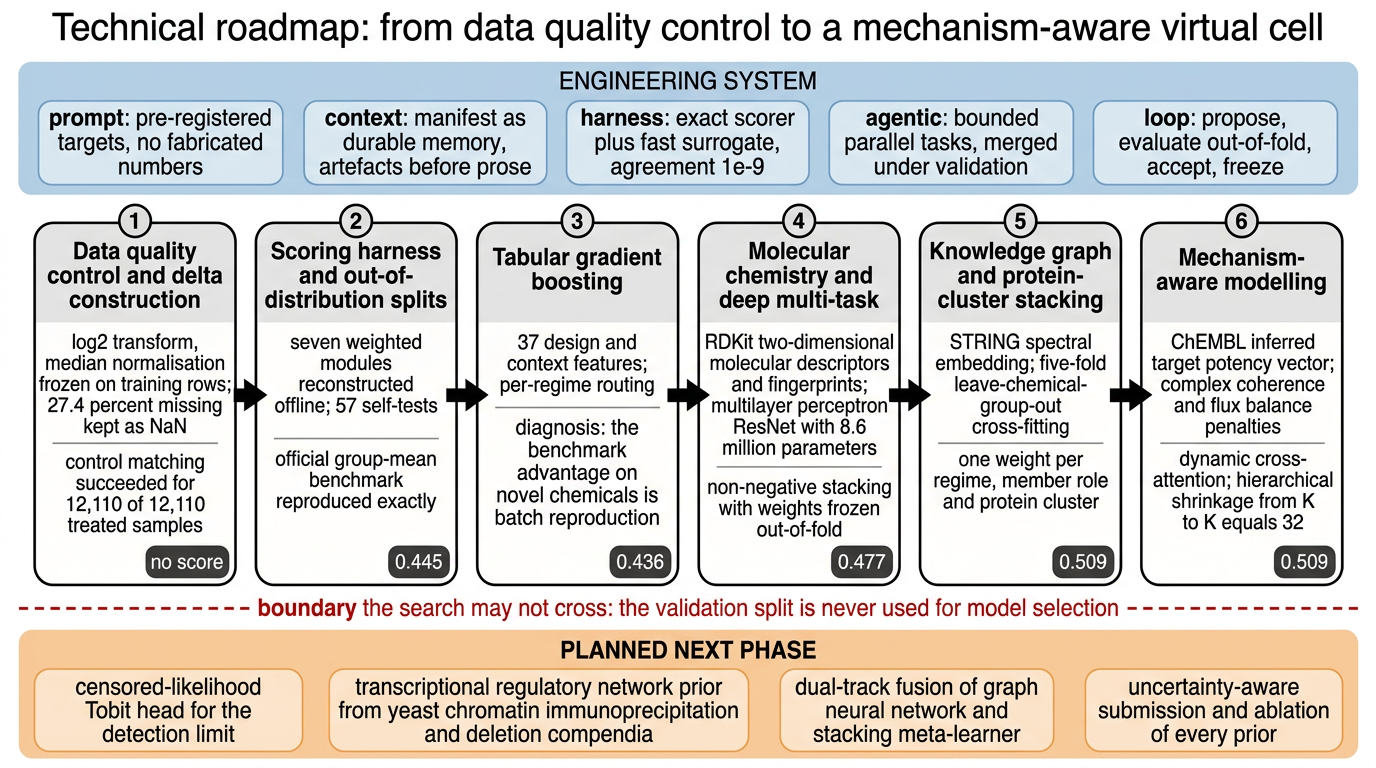
\includegraphics[width=\textwidth]{figures/roadmap.png}
\caption{\textbf{技术路线图。} 中部六个方框为已完成阶段及其\emph{验证队列}总分；上方浅蓝带为支撑这些阶段的\textbf{五层工程体系}（prompt / context / harness / agentic / loop）；下方浅橙带为复赛阶段的预注册工作。贯穿全图的红色虚线是搜索不可越界的红线：\textbf{验证集永不用于模型选择}。图中阶段 6 的「hierarchical shrinkage from $K$ to $K=32$」应读作 $K=4$ 至 $K=32$。}
\label{fig:roadmap}
\end{figure}

一句话概括架构：\textbf{一轨是端到端神经网络}（图注意力 ResNet 与动态生化交叉注意力图 Transformer），在蛋白关联图上传播扰动响应并让化学结构\emph{直接调制注意力的边}；\textbf{另一轨是结构化的分层收缩 stacking 元学习器}，在「可用性情形 $\times$ 成员角色 $\times$ 蛋白功能簇」三维张量上分配非负权重。外部知识分别以\textbf{特征、图结构与损失罚项}三种方式进入模型。

\subsection{测量层：冻结统计量与对照匹配}

log$_2$ 变换保留 NaN，逐样本中位数中心化后重对齐到\textbf{仅由训练行计算}的参照偏移 21.3286\citep{Valikangas2018Normalization}。对照匹配规则在阶段 1 即冻结：锚点为 Water 与 DMSO 合并的溶剂对照（质控注射排除），按六级上下文层级回退匹配，重复对照取中位数；培养板被\emph{刻意}排除在匹配键之外（它是 L1 键的确定性函数，纳入会把匹配粒度压到单板从而失去重复）。

实测：\code{train\_val} 7\,884 行与 \code{test} 4\,226 行\textbf{全部 12\,110 行在最细层级 \code{L1\_full\_ctx} 匹配成功，回退使用次数为零}；$\bm{\Delta}$ 定义率为 71.071\,\%（\code{train\_val}）与 70.627\,\%（\code{test}），再推导校验的最大绝对偏差为 $0.00$（覆盖 29\,377\,690 个单元）。作为反事实，若仅用 \code{train\_val} 内的对照并以板级键匹配，测试集匹配率将跌至 41.93\,\%。

\subsection{实体表征层：统一开放榜的核心}
\label{sec:entity}

统一开放榜的规则要求把「未见实体」变成「有表征的实体」。我们的六条实体轴中，\textbf{五条已有外部表征，一条仍是空白类别}（图 \ref{fig:entity}D）。这一节如实呈现两侧。

\begin{figure}[H]
\centering
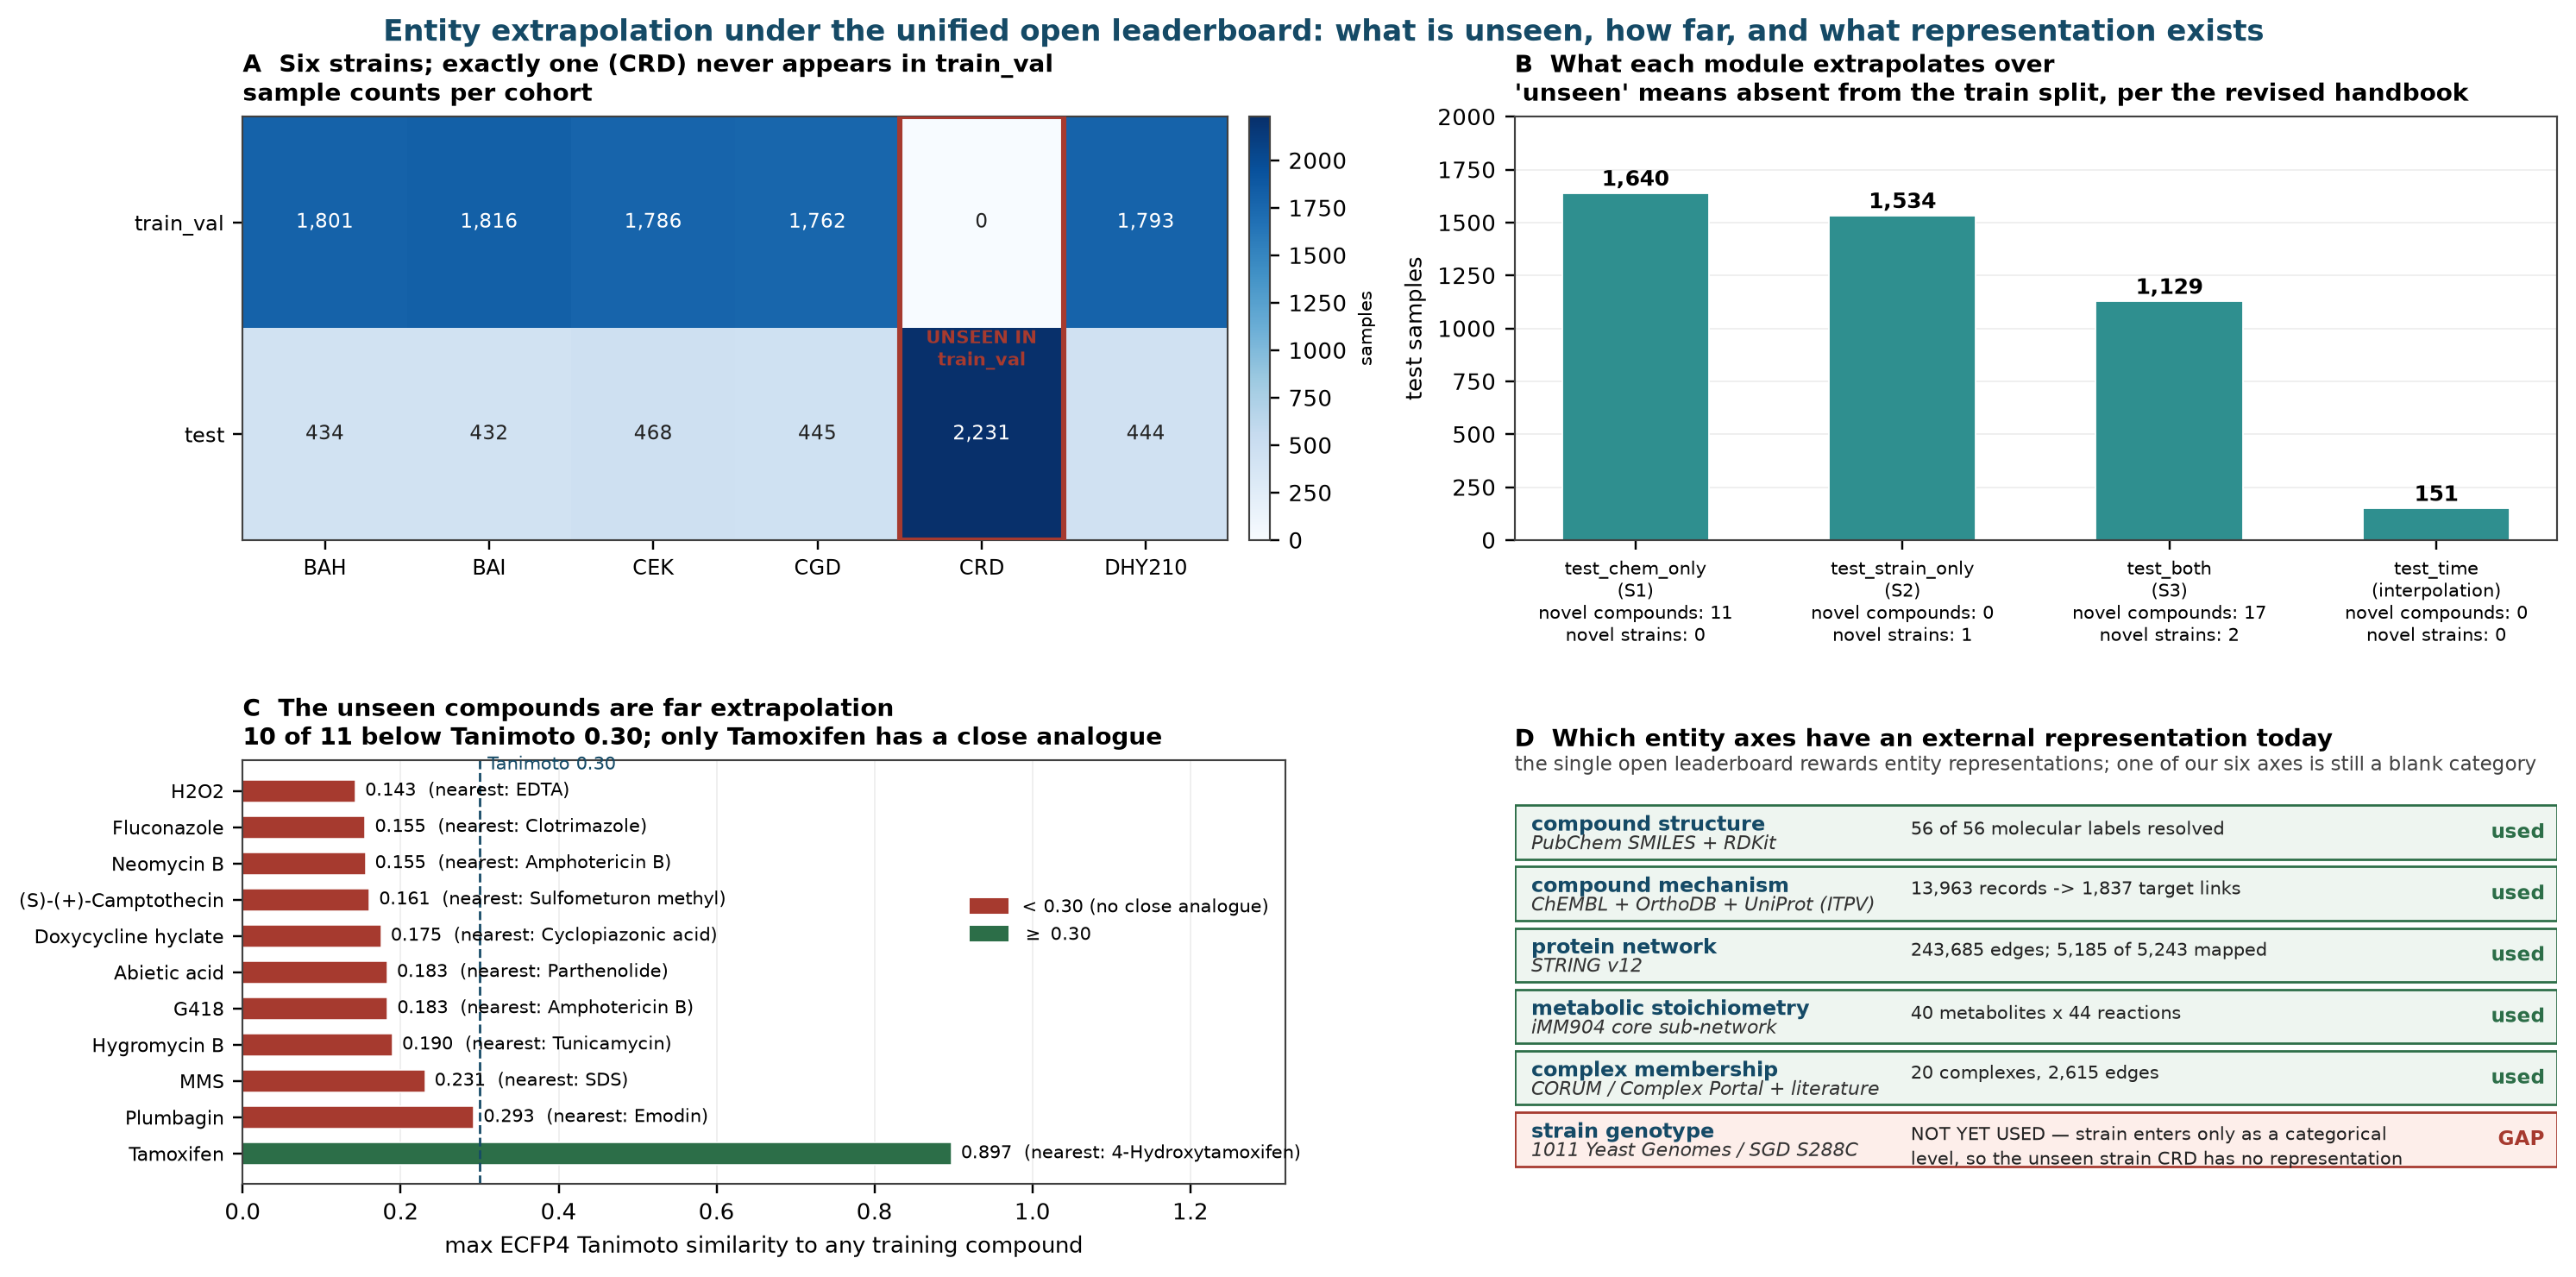
\includegraphics[width=\textwidth]{figures/step7_entity_extrapolation.png}
\caption{\textbf{统一开放榜下的实体外推图景（全部数值由结果产物在绘图时读入）。}
\textbf{A} 六个菌株在两个数据文件中的样本数，\textbf{CRD 在 \code{train\_val} 中样本数为 0}——它是唯一的未见菌株，却占测试集 2\,231 例；
\textbf{B} 四个测试划分各自外推的实体（「未见」按修订后定义：不在训练划分中）；
\textbf{C} 11 个仅在测试集出现的化合物与训练化学空间的最大 ECFP4 Tanimoto 相似度——\textbf{10 个低于 0.30}，仅他莫昔芬（0.897，近邻为 4-羟基他莫昔芬）有近似物，因此 S1 是\emph{远端}外推而非邻域插值；
\textbf{D} 六条实体轴的外部表征现状：化合物结构、化合物机制、蛋白网络、代谢化学计量、复合物成员五项已用，\textbf{菌株基因型为空白}。}
\label{fig:entity}
\end{figure}

\subsubsection{化合物结构：正是修订说明推荐的路径}

我们的化合物侧管线与修订说明推荐的路径完全一致——\textbf{通过 PubChem 检索 SMILES，使用 RDKit 生成分子描述子}\citep{kim2025pubchem,landrum_rdkit}。实测：57 个扰动标签中 \textbf{56 个解析为分子结构}（覆盖率 100.0\,\%），唯一未解析的是 \code{Quality Control}——它按修订说明本就不是化合物。所有 56 个化合物均取得 PubChem CID 与规范 SMILES，\code{source} 字段一律为 \code{pubchem}。

特征含 29 个 RDKit 二维描述子、ECFP4 指纹\citep{rogers2010ecfp}的两个变体，以及三维几何描述子（ETKDGv3 构象\citep{riniker2015etkdg} $+$ MMFF94 优化后的 Free-SASA、主惯性矩与 Gobbi 三维药效团指纹）；描述子缺失单元数为 \textbf{0}。盐析与母体分子提取经 55 个参考分子量交叉校验——这道校验捕获了两处静默失败（顺铂被还原为氨、NaCl 被剥成氯原子），二者\emph{都能正常解析}，没有该门控就是静默错误。

\subsubsection{化合物机制：推断靶点效力向量（ITPV）}

\begin{figure}[H]
\centering
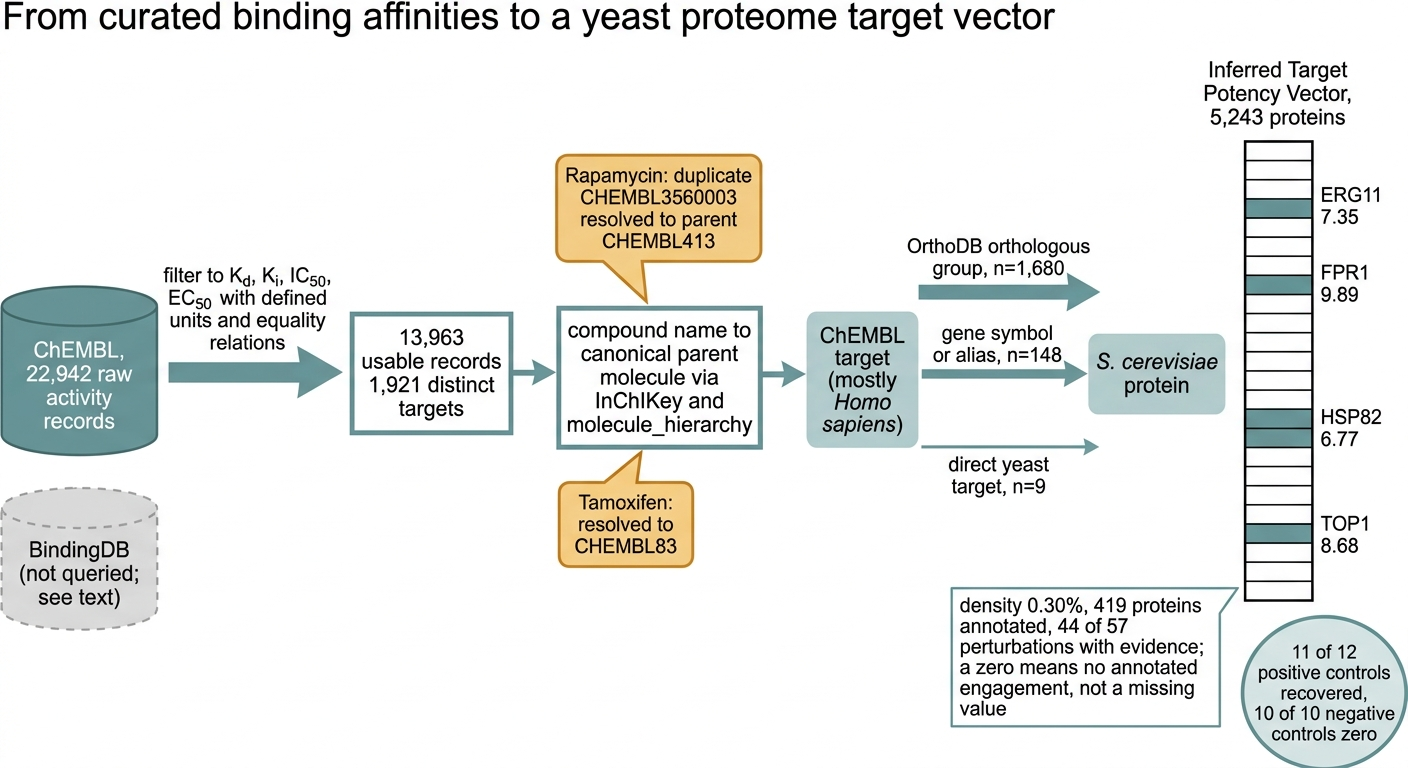
\includegraphics[width=0.93\textwidth]{figures/paper6_itpv_mapping.png}
\caption{\textbf{推断靶点效力向量（ITPV）的构造。} 化合物先解析到 ChEMBL \textbf{规范母体分子}（这一步的遗漏曾使机制覆盖率减半且不抛错）；从 22\,942 条原始记录保留 13\,963 条可解释、未删失的 $K_d/K_i/\mathrm{IC}_{50}/\mathrm{EC}_{50}$ 记录，跨 1\,921 个靶点、1\,057 个 UniProt 登录号\citep{mendez2019chembl,uniprot2025}；再经三条可靠性递减的通道投射到被测酵母蛋白轴——OrthoDB 直系同源组 1\,680 条、基因符号一致 148 条、靶点本身即酵母蛋白 9 条，共 \textbf{1\,837 条连边}。得到的 5\,243 维稀疏向量非零密度 0.299\,\%，覆盖 44 个扰动与 419 个蛋白；\textbf{零元断言「无注释接合」而非缺失，永不填补}，且携带 \code{has\_chembl\_evidence} 指示位以区分「无靶点」与「未查询」。该矩阵再由仅用 37 个训练化合物拟合的截断 SVD 压缩为 24 维（累计解释方差 99.44\,\%）。}
\label{fig:itpv}
\end{figure}

\begin{okbox}[title=先验的独立验证（事先声明的药理学对照）]
\small
阳性侧：12 个化合物中 \textbf{11 个被召回}（21 对关系中 20 对带注释），唯一失败为 4-羟基他莫昔芬 $\to$ ERG2（数据源无该注释）。特别值得注意的是雷帕霉素——其效力被正确映射到 \textbf{FPR1}（FKBP12 同源物）而\emph{不是}直接映射到 TOR，这与「雷帕霉素-FKBP12 复合物才是 TOR 抑制的实际形式」这一药理学事实一致。
阴性侧：10 组对照\textbf{全部为零}。阴性对照是这项检验中信息量更大的一半——一个过度泛化的映射会在此失败。
\textbf{预期是在读矩阵之前、按每个化合物的机制写下的}，而不是事后从矩阵里读出来的。
\end{okbox}

\subsubsection{蛋白网络、复合物与代谢化学计量}

\textbf{（一）蛋白关联网络。} STRING v12.0（taxon 4932，置信度 $\ge400$）提供 243\,685 条无向边，5\,243 个蛋白中 5\,185 个成功映射（最大连通分量 5\,171 节点、72 孤立点）\citep{szklarczyk2023string}。我们从归一化 Laplacian 提取 64 维谱嵌入\citep{belkin2003laplacian,vonluxburg2007tutorial}，与\emph{仅用训练行}计算的丰度统计量拼接后 $K$-means 聚类，得到元学习器所需的蛋白功能簇。一致性检查：训练集内共响应图（$k=20$ 近邻，95\,752 条边）与 STRING 图的 Jaccard 相似度仅 \textbf{0.0324}——两张图携带互补而非冗余的信息，与复合物成员共调控的既有观察一致\citep{kustatscher2019coregulation}。

\textbf{（二）复合物共调控。} 脚本以 CORUM、Complex Portal 与酵母复合物文献\citep{tsitsiridis2023corum,meldal2022complexportal}为背景，\textbf{手工编码} 20 个复合物的成员名册（60S/40S 核糖体、19S/20S 蛋白酶体、SAGA、RNA 聚合酶 I/II/III、TRiC、V-ATPase、F$_1$F$_0$-ATP 合酶、eIF3、TFIID、外切体、COPI/COPII、HSP90 系统、MCM、CCR4-NOT 等）。这不是数据库导出，当前公开产物也未保留逐边来源字段；可核查的范围是脚本常量、20/20 个复合物至少有 2 个被测亚基，以及由此生成的 \textbf{2\,615 条}共复合物边。每条边按 $1/(k-1)$ 加权，使大复合物按亚基数而非按二次增长的配对数贡献。

\textbf{（三）代谢化学计量。} 以已发表的 iMM904 重构\citep{mo2009imm904}为文献依据，脚本\textbf{手工编码 iMM904 风格的核心子网络}，而非读取或裁剪一个随仓库发布的 iMM904 模型文件。该子网络含 \textbf{44 个反应、40 个被平衡代谢物}（化学计量矩阵 $40\times44$），覆盖糖酵解/发酵、TCA、磷酸戊糖途径与\textbf{麦角固醇生物合成}，\textbf{全部 44 个反应至少有一个被测酶}\citep{orth2010fba,heirendt2019cobra}；仅接触少于 2 个保留反应的死端代谢物被剔除。当前可复核的是编码表和数值验证，不能把它表述为完整上游模型的逐项再发布。

\subsubsection{\NEW{}尚未补齐的一条轴：菌株基因型}

必须明确写出：\textbf{本次提交的模型没有使用任何菌株基因组特征}。菌株仅以类别变量与若干以菌株为键的目标编码进入模型，因此对未见菌株 CRD 而言，\emph{它在推断时确实是一个空白类别}——所有以菌株为键的特征族在 S2 划分上定义率为 0，模型只能依靠测量上下文（批次与仪器为键的特征族仍保有 0.912 与 0.906 的定义率）与全局响应结构。

这解释了一个此前难以解释的现象：我们在 S2 上相对基线的增益（测试队列 0.3278 对 0.2905）明显小于在 TIME 上的增益（0.5599 对 0.4378）。修订说明第一条的论证在我们身上直接命中，我们把它作为下一阶段的\textbf{第一优先工作项}（表 \ref{tab:plan} 工作项 E），拟用 1011 酵母基因组项目\citep{peter2018_1011genomes}的变异集构造菌株表征，并以 SGD S288C 参考基因组\citep{engel2022sgd}作为 DHY210 的代理——这正是修订说明推荐的两个来源。判据事先写下：\emph{S2 模块提升 $\ge0.010$，且在 embedding 打乱对照下增益必须消失}。后半句是关键——如果打乱菌株嵌入后分数不掉，那么涨的不是基因组信息。

\begin{table}[H]
\centering\small
\caption{\textbf{外部公开资源的来源、版本与许可披露（修订第二条与第四条要求）。} 本表与 \file{workflow/51\_external\_data\_manifest.py}、公开快照 \file{evidence/step7\_external\_data\_manifest.json} 同步。「未记录」表示原始产物没有保存足以追溯精确发布号的信息，本文不作事后猜测。「影响成绩」指若移除该资源或手工先验，本方案报告的分数是否改变。}
\label{tab:external}
\begin{tabularx}{\textwidth}{@{}R{2.35cm}R{3.0cm}R{2.5cm}Xc@{}}
\toprule
\textbf{资源} & \textbf{版本 / 获取} & \textbf{许可} & \textbf{用途与实测计数} & \textbf{影响\newline 成绩} \\
\midrule
\textbf{PubChem}\newline（推荐源） & PUG-REST，2026-08-05 & 依上游记录而异，\textbf{非统一公有领域} & 化合物 SMILES 与 CID；\textbf{56/56} 分子标签解析，覆盖率 100.0\,\% & 是 \\
\textbf{RDKit}\newline（推荐源） & 2026.03.5 & BSD-3 & 29 个二维描述子、ECFP4、ETKDGv3 $+$ MMFF94 三维描述子；缺失单元 0 & 是 \\
ChEMBL & Web 服务，2026-08-07；\textbf{发布号未记录} & \textbf{CC BY-SA 3.0} & 22\,942 条原始记录 $\to$ 13\,963 条可用；1\,921 靶点、1\,057 UniProt 登录号 & 是 \\
OrthoDB & UniProt REST 返回的交叉引用；\textbf{子版本未记录} & 上游条款未随产物留存 & 直系同源通道 1\,680 条；并有符号 148、直接 9，共 1\,837 条 & 是 \\
UniProt & REST，2026-08-07；\textbf{发布头未留存} & CC BY 4.0 & 登录号、基因符号与 OrthoDB 交叉引用规范化 & 是 \\
STRING & \textbf{v12.0}，taxon 4932，score $\ge400$ & CC BY 4.0 & 243\,685 条无向边；5\,185/5\,243 映射；64 维谱嵌入 & 是 \\
iMM904 & Mo 等（2009）文献启发 & 未分发第三方模型文件 & 手工编码的 40 代谢物 $\times$ 44 反应子网；44/44 反应有被测酶 & 是 \\
CORUM /\newline Complex Portal / 文献 & 手工成员名册；非数据库导出 & 未分发上游记录；逐边来源未保留 & 20 个复合物、2\,615 条共复合物边 & 是 \\
\midrule
\textbf{1011 酵母\newline 基因组}\newline（推荐源） & \file{1002genomes.u-strasbg.fr/files/} & 使用前须复核具体数据条款 & \textbf{计划使用，当前未使用}：未见菌株 CRD 的实体表征 & \textbf{否} \\
\textbf{SGD S288C}\newline（推荐源） & SGD 参考基因组 & 使用前须复核具体数据条款 & \textbf{计划使用，当前未使用}：DHY210 的代理参考 & \textbf{否} \\
\midrule
官方竞赛数据 & 官网发布四文件 & 赛事数据使用协议 & 训练与评测；\textbf{仅限本次竞赛，不再分发} & 是 \\
\bottomrule
\end{tabularx}
\end{table}

\subsection{机制受限的损失函数}

复合物一致性与代谢化学计量两项先验以\textbf{机制损失}进入目标函数：
\begin{equation}
\mathcal{L}=\underbrace{w_{\text{mse}}\mathcal{L}_{\text{mse}}}_{1.0}
+\underbrace{w_{\text{pcc}}\mathcal{L}_{\text{pcc}}}_{0.5}
+\underbrace{w_{\text{cx}}\sum_{c}\sum_{(u,v)\in E_c}\tfrac{1}{k_c-1}(\hat{\Delta}_u-\hat{\Delta}_v)^2}_{0.02}
+\underbrace{w_{\text{flux}}\lVert\mathbf{S}\bm{v}(\hat{\bm{\Delta}})\rVert_2^2}_{0.01},
\label{eq:mechloss}
\end{equation}
其中 $\mathcal{L}_{\text{mse}}$ 为掩码均方误差（有限交集掩码，缺失不参与），$\mathcal{L}_{\text{pcc}}=1-\overline{\operatorname{PCC}}_{\text{sample}}$，$\mathbf{S}\in\mathbb{R}^{40\times44}$ 为化学计量矩阵，$\bm{v}$ 为通量代理（取反应催化酶预测 log$_2$ 倍数变化的均值，即标准的酶容量代理）。两项机制罚项系数刻意取小，角色是\textbf{弱正则而非硬约束}，与物理信息神经网络中软约束的通行做法一致\citep{karniadakis2021pinn}。四个损失项均与独立实现的 NumPy 参考逐项比对，最大绝对偏差 $4.88\times10^{-6}$（容差 $10^{-3}$）。

\begin{figure}[H]
\centering
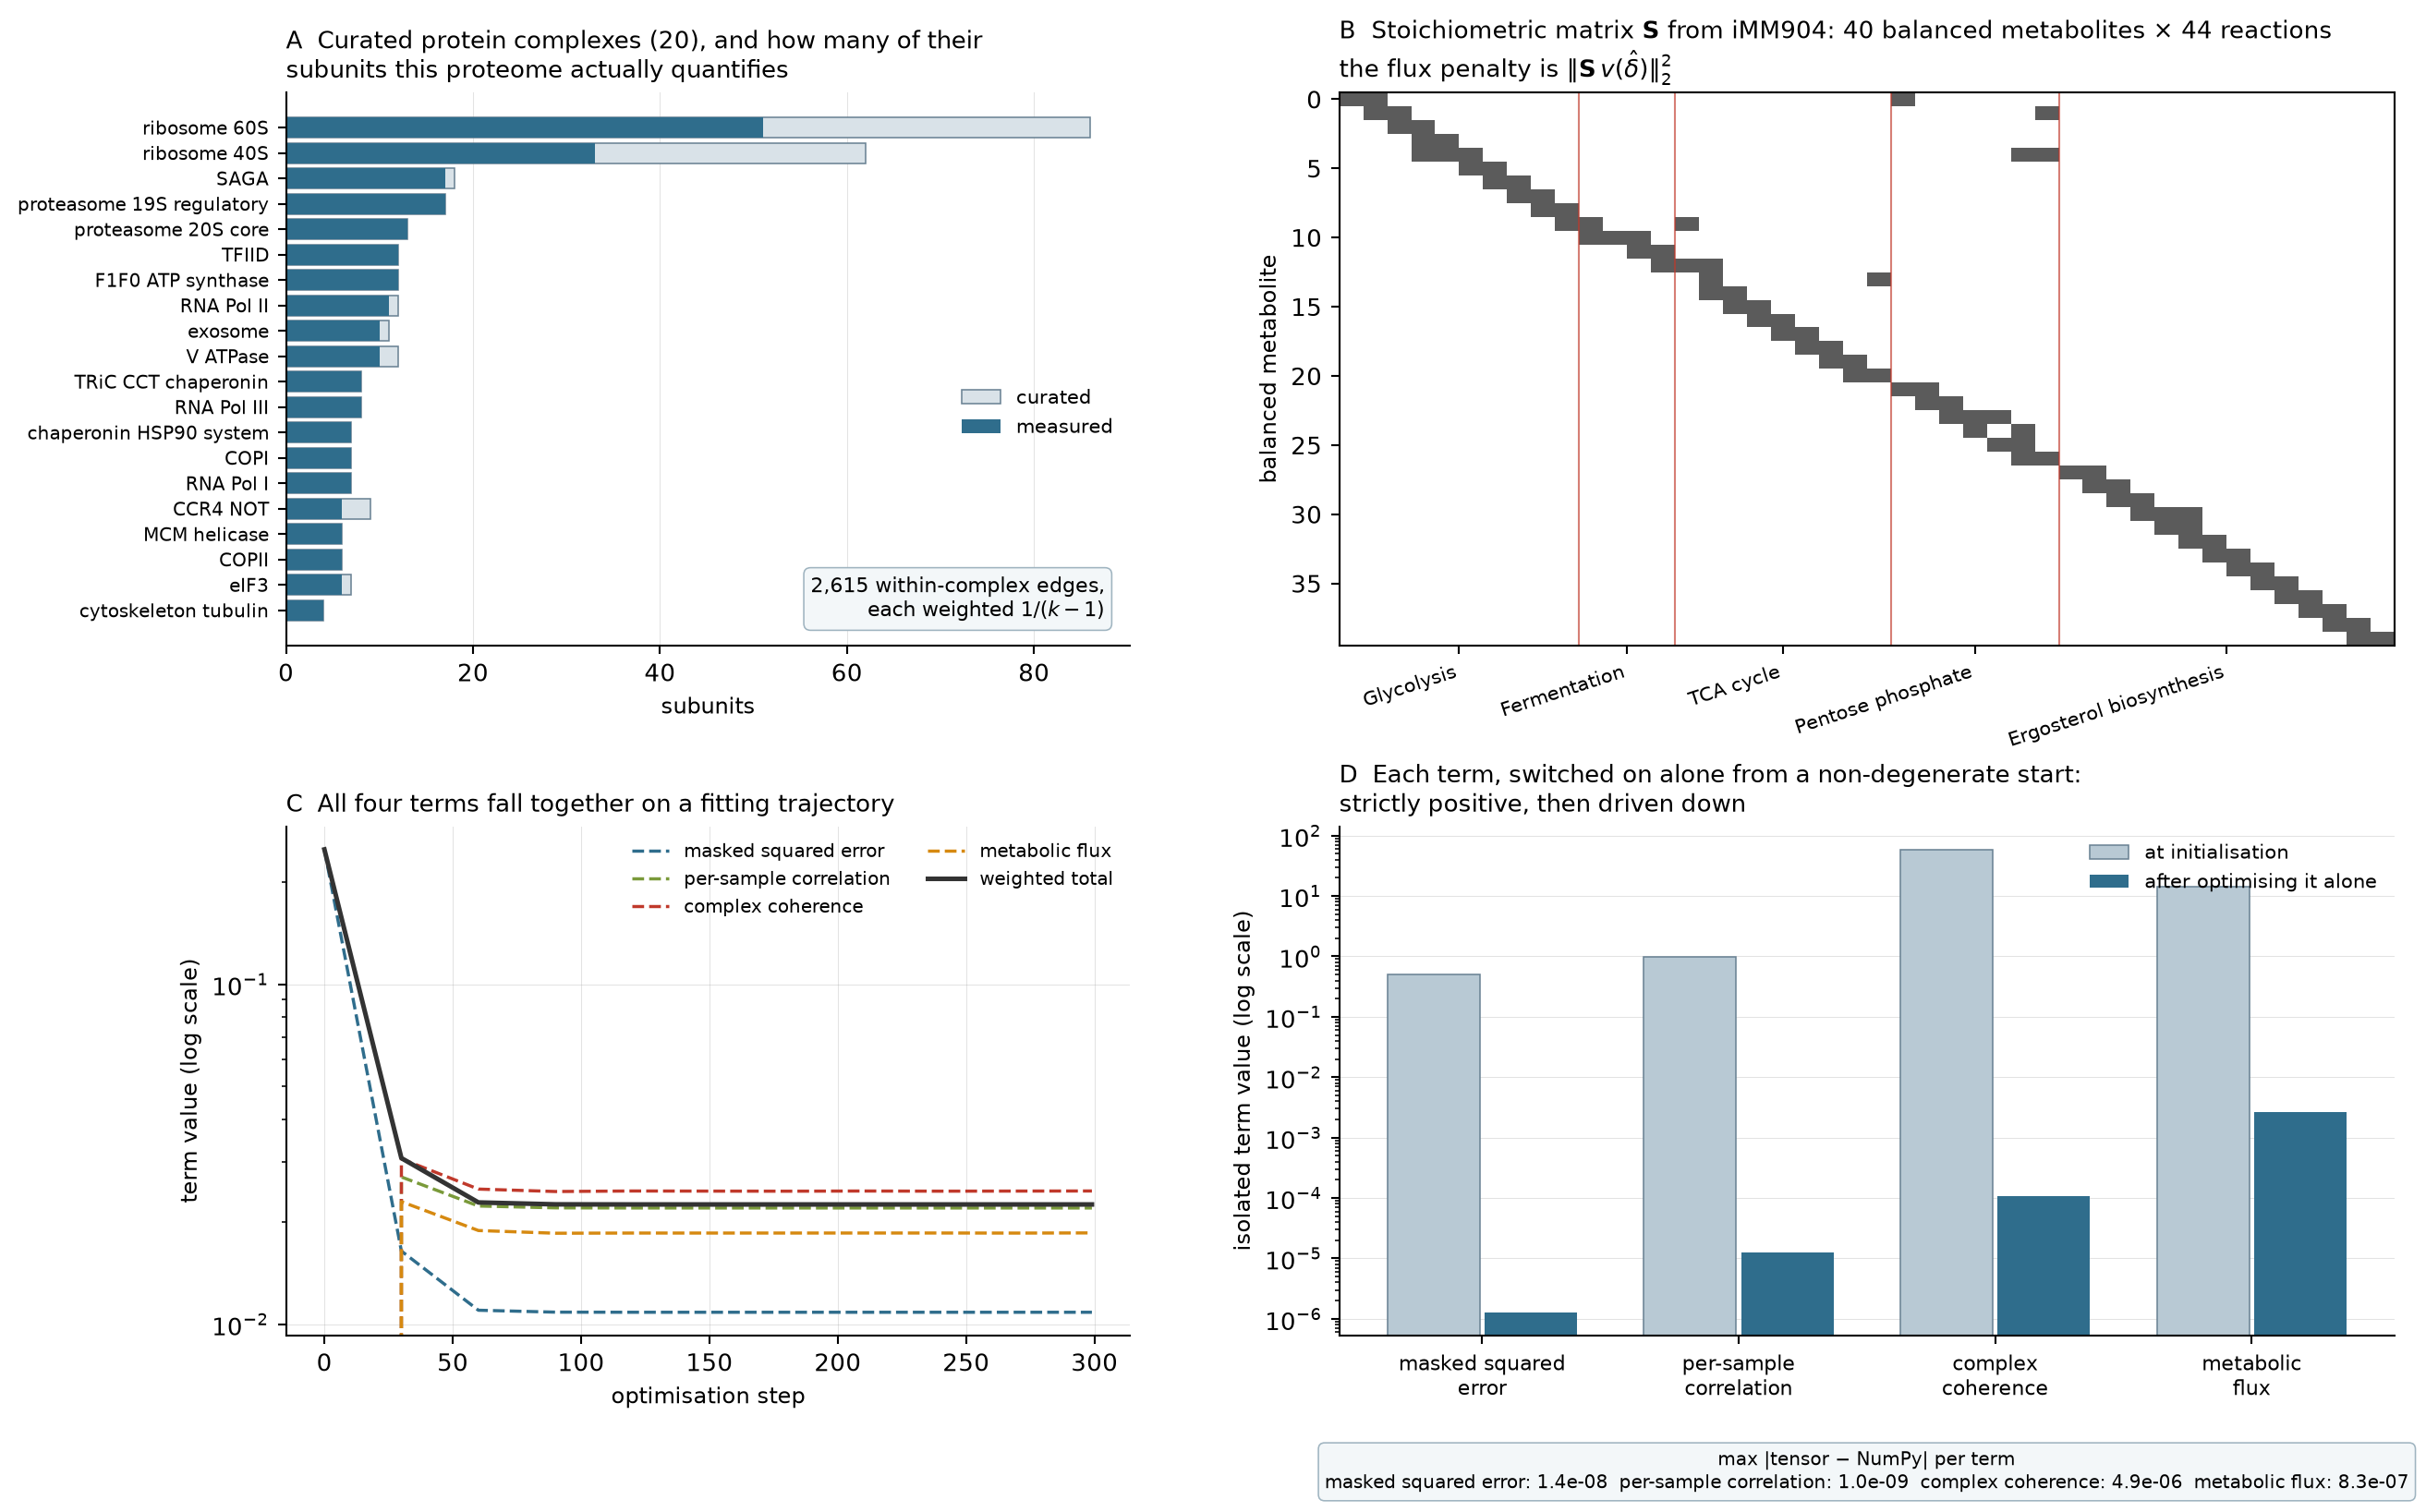
\includegraphics[width=0.95\textwidth]{figures/step6_mechanism_loss_detail.png}
\caption{\textbf{机制损失的数值验证（四个面板全部由结果产物在绘图时读入）。}
\textbf{A} 20 个人工整理的蛋白复合物及其被测亚基数；
\textbf{B} 取自 iMM904 的化学计量矩阵 $\mathbf{S}$（40 个被平衡代谢物 $\times$ 44 个反应）；
\textbf{C} 一条拟合轨迹上四个损失项同时下降；
\textbf{D} 每个项从\emph{非退化初值}单独开启时的下降曲线——用以确认\textbf{每一项都真实起作用}，而非被其他项的下降所掩盖。四项与独立 NumPy 参考实现的最大绝对偏差为 $4.88\times10^{-6}$（容差 $10^{-3}$）。}
\label{fig:mechloss}
\end{figure}

\subsection{成员层：梯度提升与图注意力双轨}

\textbf{表格与分子成员。} 使用 37 个设计与上下文特征，并按四种可用性情形（已见 / 新化合物 / 新菌株 / 双新）分别训练专家模型，再按样本的实体可见性路由。必须路由，是因为不同情形可用的特征族不同：S1 上所有以化合物为键的目标编码定义率为 0；S2 上以\emph{菌株}为键的特征族定义率为 0，而以批次与仪器为键的特征族仍保有 0.912 与 0.906——S2 上失去的是菌株身份而非测量上下文。梯度提升在此类异质表格数据上的优势有充分经验支持\citep{ke2017lightgbm,chen2016xgboost,prokhorenkova2018catboost,grinsztajn2022why}，目标编码的泄漏风险以折外编码规避\citep{miccibarreca2001preprocessing,kaufman2011leakage}。

\begin{figure}[H]
\centering
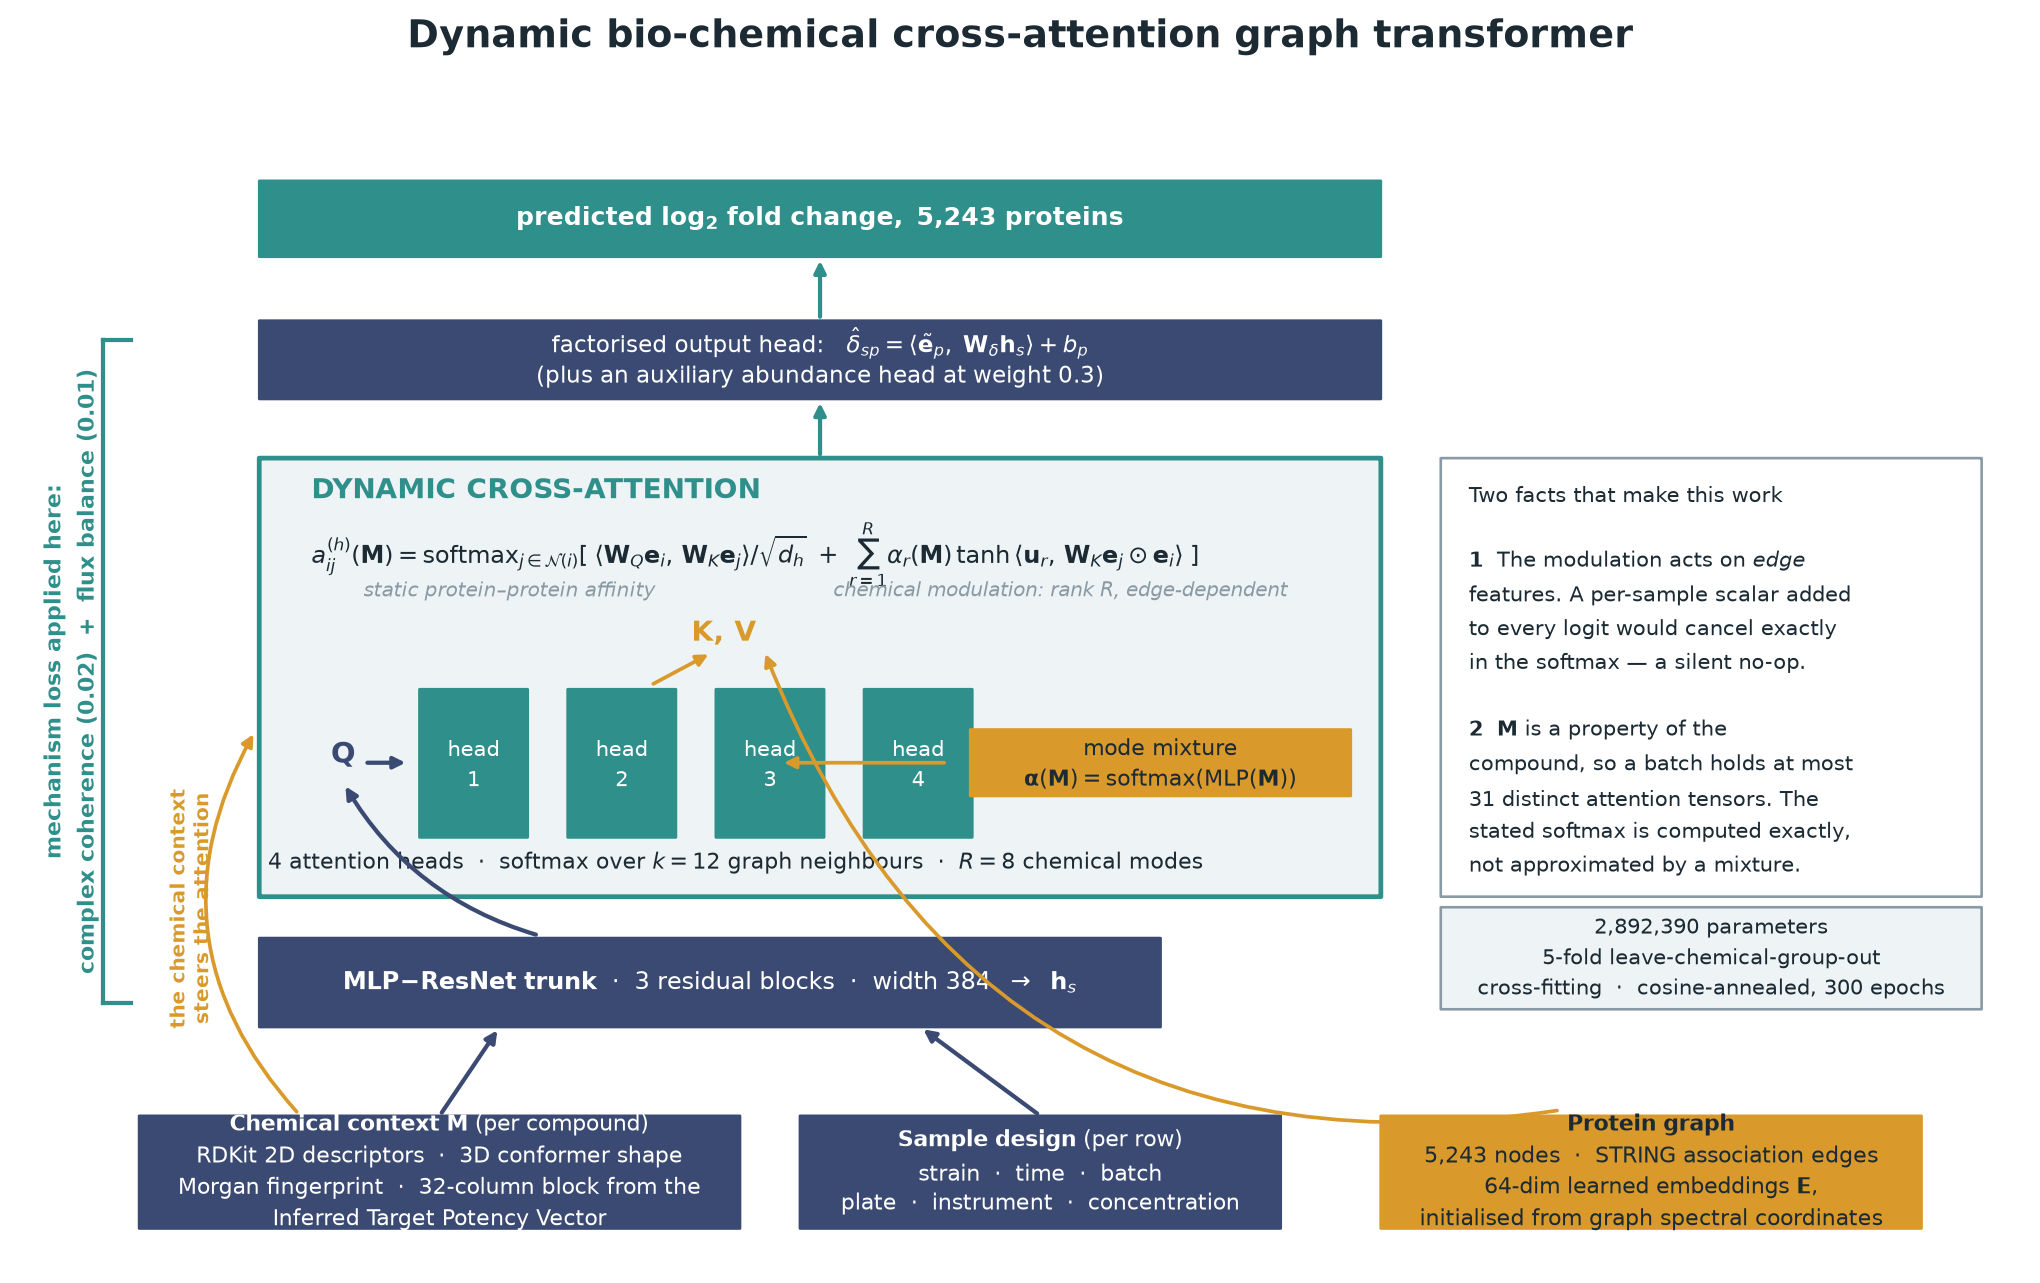
\includegraphics[width=0.95\textwidth]{figures/step6_xattn_architecture.png}
\caption{\textbf{动态生化交叉注意力图 Transformer（计数由训练产物在绘图时读入）。} 化学上下文与样本设计向量经 MLP-ResNet 主干后进入交叉注意力模块，注意力对数由\emph{静态蛋白-蛋白亲和}加上\emph{化学调制}构成，在 $k=12$ 的 STRING 邻域上归一化，输出经因子化多任务头给出 5\,243 维 log$_2$ 倍数变化。参数量随折在 2\,892\,006--2\,892\,390 之间，五折留化学组交叉拟合、余弦退火 300 轮、折外覆盖率 1.0、五折平均最优开发 PCC 0.2075。}
\label{fig:xattn}
\end{figure}

\textbf{图神经成员。} 阶段 5 为在蛋白输出头受 STRING 邻接 Laplacian 平滑罚 $\operatorname{tr}(\mathbf{P}^\top\mathbf{L}\mathbf{P})$ 正则的图注意力 ResNet\citep{velickovic2018graph,kipf2017gcn,he2016deep}，五折平均最优开发 PCC 0.2109。阶段 6 引入动态生化交叉注意力（图 \ref{fig:xattn}），核心是让化学上下文调制注意力的\emph{边}特征：
\begin{equation}
a^{(h)}_{uv}(m)=\frac{\exp\!\big(e^{(h)}_{uv}+\bm{\phi}(m)^\top\bm{\psi}^{(h)}_{uv}\big)}{\sum_{v'\in\mathcal{N}_k(u)}\exp\!\big(e^{(h)}_{uv'}+\bm{\phi}(m)^\top\bm{\psi}^{(h)}_{uv'}\big)},
\label{eq:xattn}
\end{equation}
$e^{(h)}_{uv}$ 为静态蛋白亲和对数，$\bm{\phi}(m)$ 为化合物的 59 维化学上下文向量（含 ITPV 压缩块 24 维），$\bm{\psi}^{(h)}_{uv}$ 为可学习的边调制基（8 个化学模式，4 个注意力头）。这一细节是必要的：\textbf{softmax 是平移不变的，若调制项只依赖 $u$ 而不依赖 $v$，它会恒等地约掉}，架构退化为静态注意力。

\subsection{元学习层：蛋白簇分层收缩 stacking}

\begin{figure}[H]
\centering
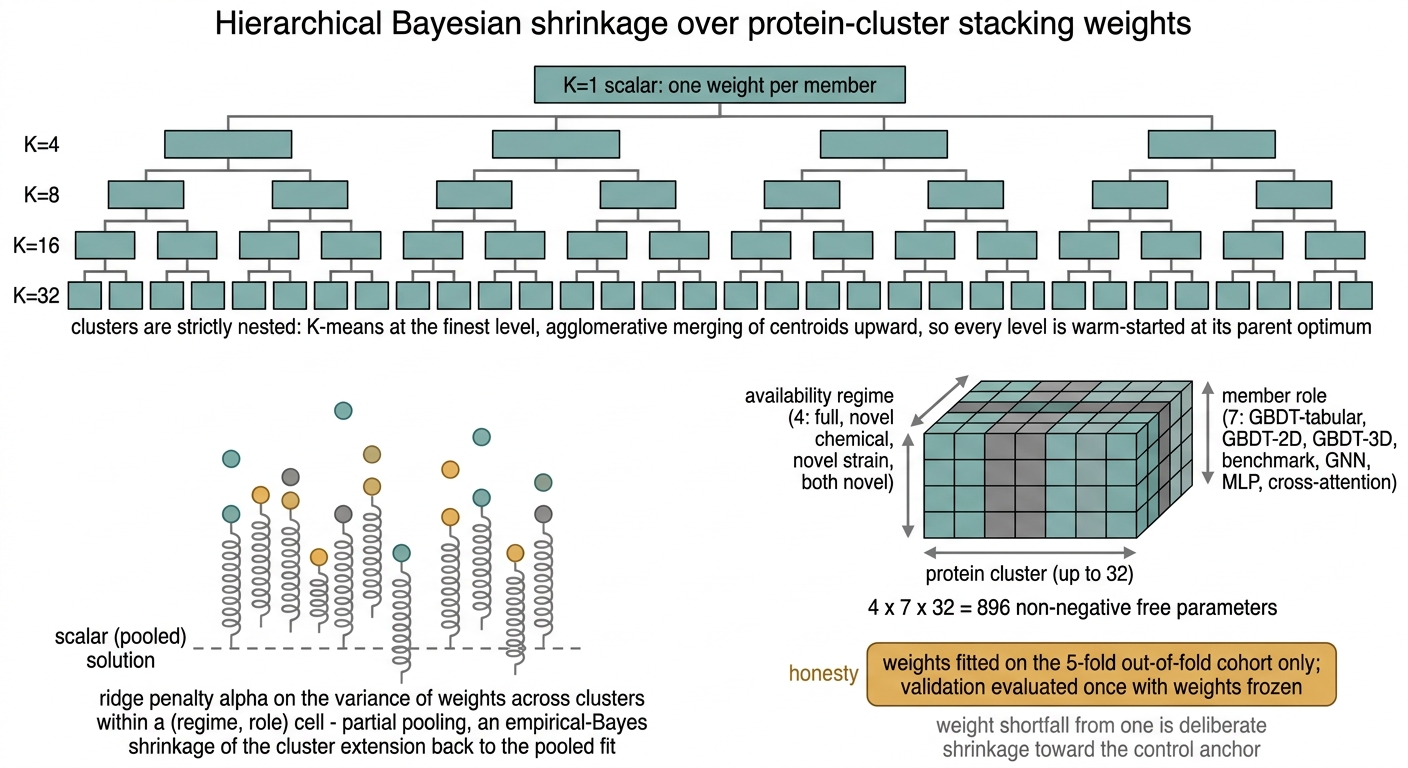
\includegraphics[width=0.90\textwidth]{figures/paper6_hierarchical_shrinkage.png}
\caption{\textbf{蛋白簇分层收缩 stacking。} 元学习器把标量权重扩展为三维非负张量 $\mathbf{W}\in\mathbb{R}_{\ge0}^{R\times M\times C}$（情形 $\times$ 角色 $\times$ 蛋白簇）。动机来自评分口径本身：Module 1 含两个 $R^2$ 项与一个逐蛋白均值 PCC 项，因此向对照锚点收缩的\emph{最优程度是蛋白相关的}——高丰度代谢酶容许较大的 $\Delta$，低丰度调控因子则不容许。簇划分严格嵌套（$K=4\!\to\!8\!\to\!16\!\to\!32$），每层在父层最优点热启动，并施加跨簇方差罚把权重拉向池化解。\textbf{权重之和刻意允许小于 1：缺口不是松弛，而是向对照锚点的显式收缩。} 图中标注的 $4\times7\times32=896$ 为名义上限，实际最细层实现 31 个簇、\textbf{868 个自由参数}。}
\label{fig:hier}
\end{figure}

元学习器的优化目标为
$\min_{\mathbf{W}\ge0}\;-\mathcal{S}_{\text{OOF}}(\mathbf{W})+\alpha\sum_{r,m}\operatorname{Var}_c(W_{rmc})$，
其中 $\mathcal{S}_{\text{OOF}}$ 为\textbf{折外}队列上的加权总分。该构造是分层收缩的直接应用\citep{gelmanhill2006multilevel,efron1975stein}，非负性由构造保证\citep{bro1997fnnls}。权重校准队列由\textbf{五折留化学组交叉拟合}（LCGO）给出：化合物按行数均衡分 5 组，第 $f$ 折的拟合集为「化学组 $\ne f$ 且菌株组 $\ne f$」的行，使每个开发折同时含四种可用性情形；泄漏审计 5 项逐折断言全部通过。这把校准队列由阶段 4 的 2\,700 行扩到全部 5\,078 行，其统计动机见堆叠泛化\citep{wolpert1992stacked,breiman1996stacked,vanderlaan2007super}与交叉拟合去偏\citep{chernozhukov2018double}文献。最终选中配置为 \code{cluster\_column = k32}、$\alpha=0$，\textbf{选择队列仅为折外队列，验证集未被查询}。

\begin{figure}[H]
\centering
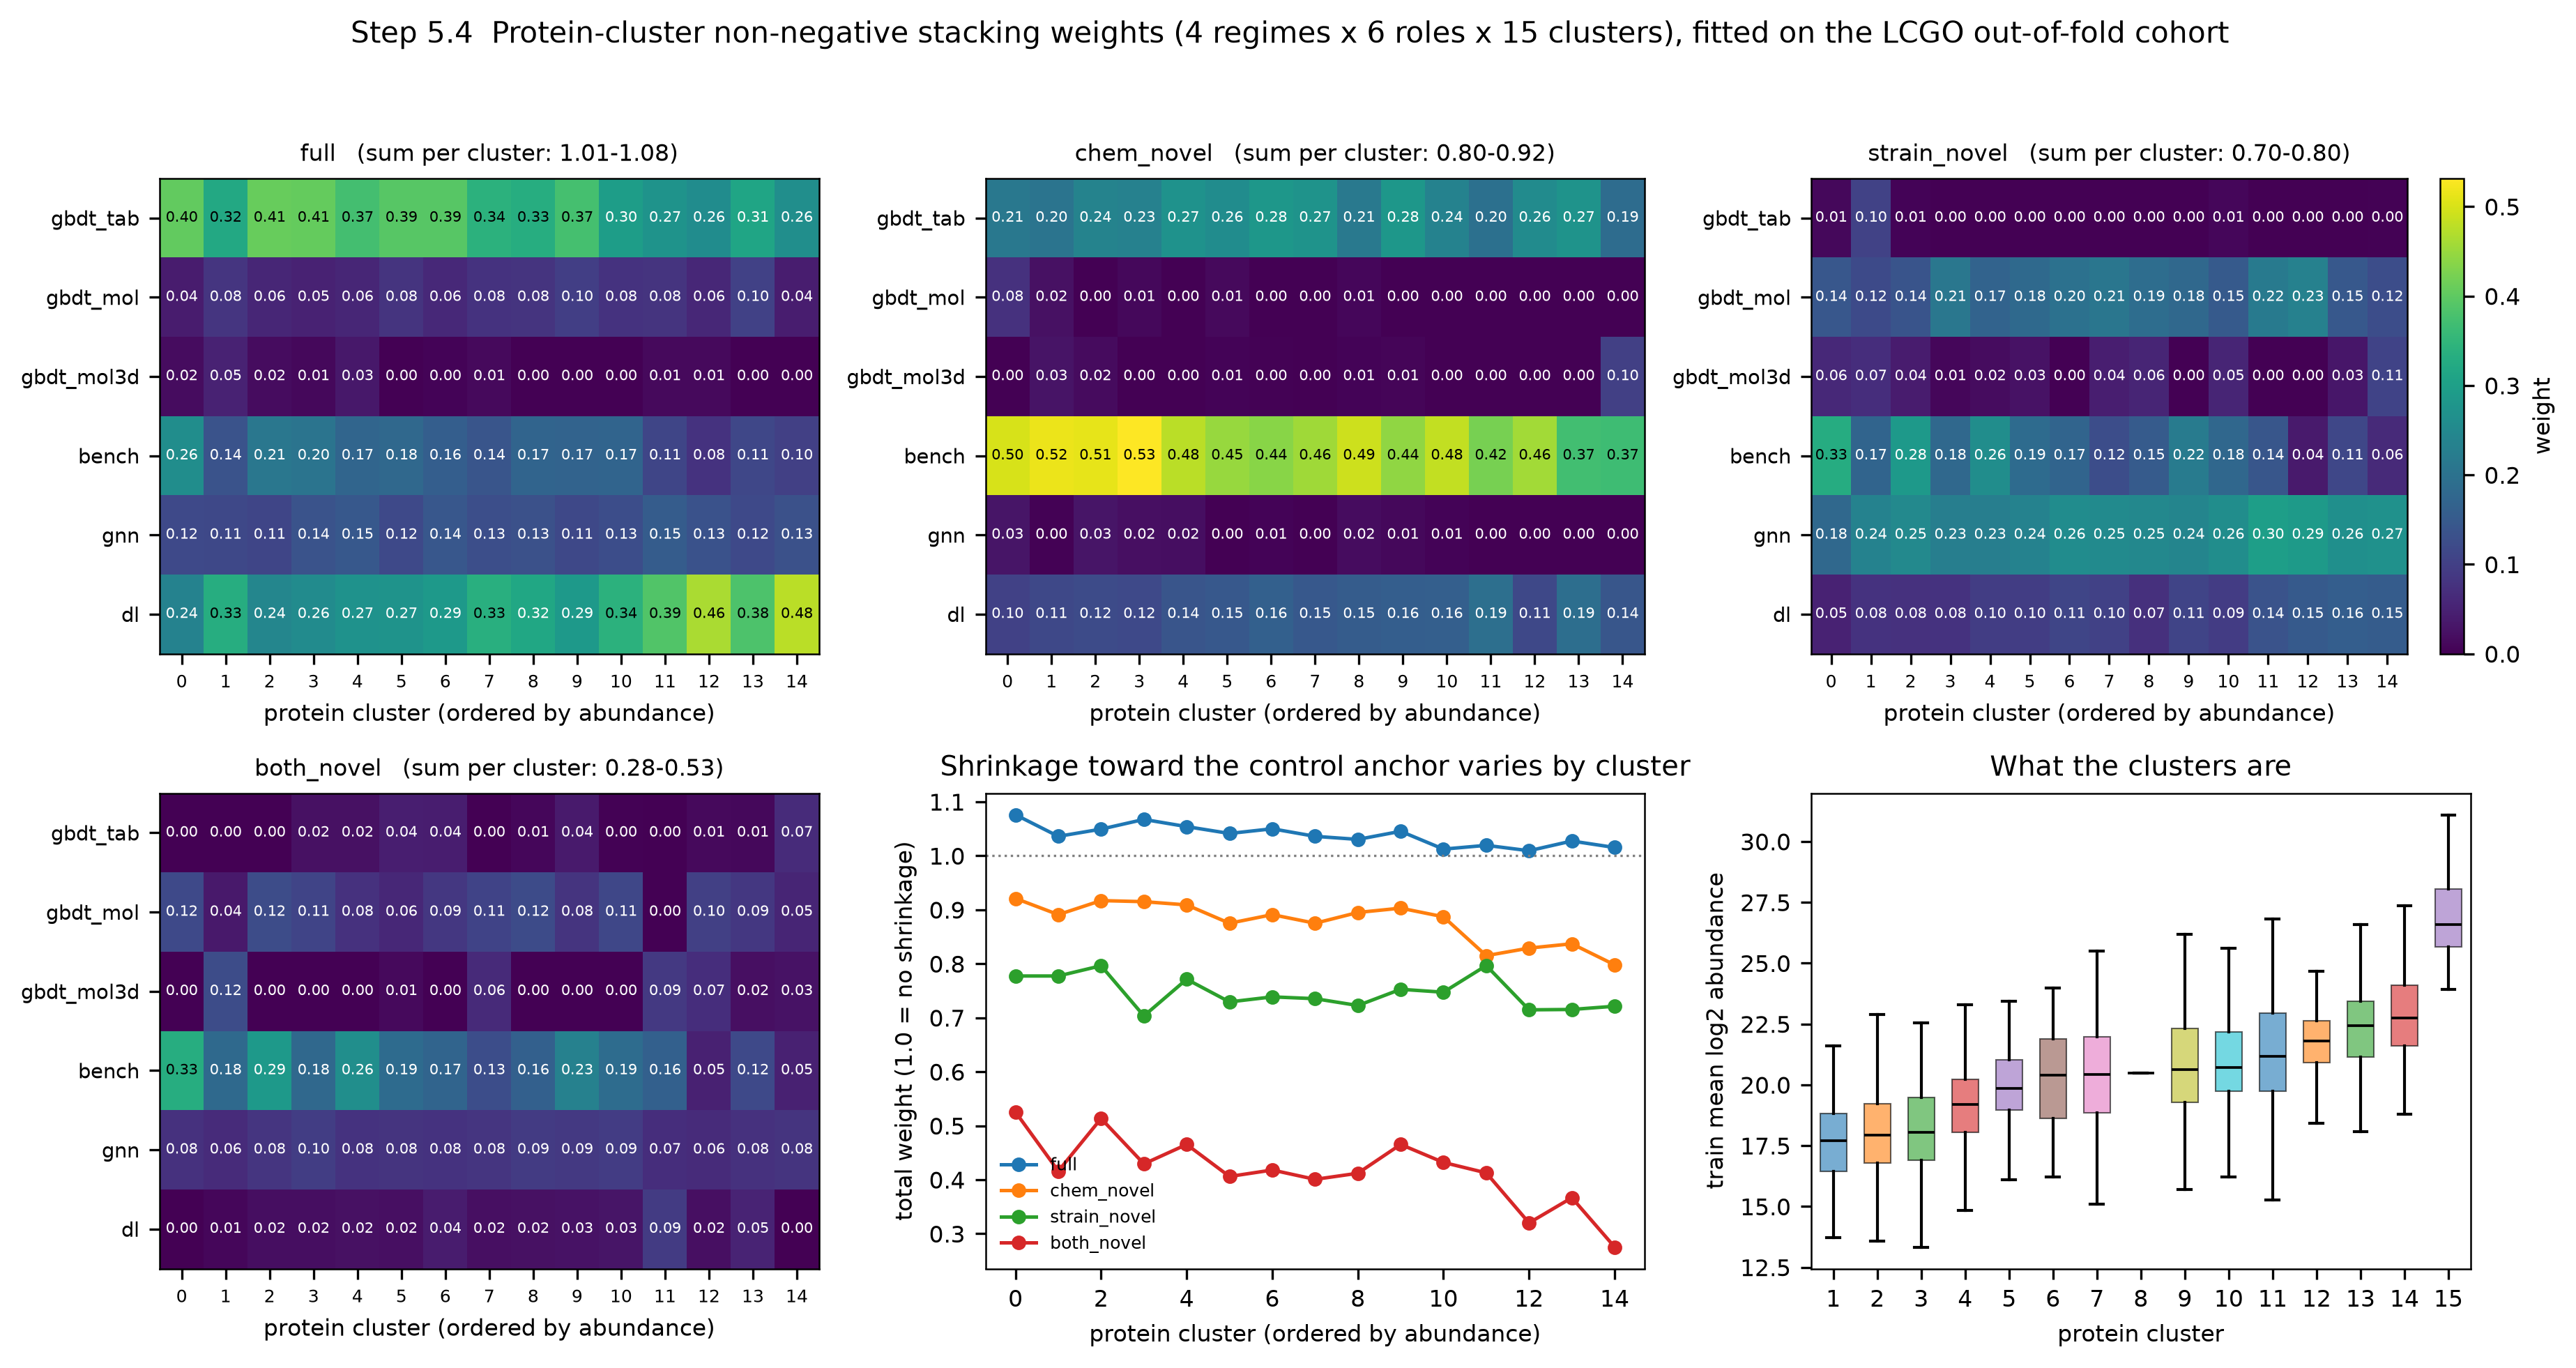
\includegraphics[width=0.95\textwidth]{figures/step5_cluster_stacking_weights.png}
\caption{\textbf{蛋白簇非负堆叠权重张量。} 上排与左下的四张热图分别对应四种可用性情形（行为成员角色、列为蛋白功能簇）；右下两张给出逐簇权重总和与各簇的丰度分布。\textbf{权重之和小于 1 的缺口不是松弛，而是显式收缩——在响应幅度小的簇上收缩更强}，这正是「最优收缩程度是蛋白相关的」这一判断的直接可视化，也是本方案相对标量 stacking 取得增益的机制所在。}
\label{fig:weights}
\end{figure}

\subsection{左删失与 Tobit 似然（下一阶段预注册）}
\label{sec:tobit}

设蛋白 $p$ 在样本 $i$ 的潜在真实丰度 $z_{ip}$、检出限 $\tau_p$，则在 $z_{ip}\sim\mathcal{N}(\hat y_{ip},\sigma_p^2)$ 下的删失似然即经典 Tobit 模型\citep{Tobin1958LimitedDependent,Amemiya1984Tobit}：
\begin{equation}
\ell_{ip}=
\begin{cases}
-\log\sigma_p-\dfrac{(y_{ip}-\hat y_{ip})^2}{2\sigma_p^2}, & \text{检出},\\[7pt]
\log\Phi\!\left(\dfrac{\tau_p-\hat y_{ip}}{\sigma_p}\right), & \text{未检出}.
\end{cases}
\label{eq:tobit}
\end{equation}
其含义是：对未检出单元，模型不再被要求匹配某个被填补的数值，而只被要求\textbf{把预测压到检出限之下}——这恰是数据所支持的全部信息。该思路在质谱蛋白质组学统计框架中已有先例\citep{Karpievitch2009StatFramework}。

\begin{warnbox}[title=诚实边界：已验证的结果 vs. 预期的方法路线]
\small
截至本次提交，\textbf{已训练的全部模型使用式 \eqref{eq:mechloss} 的掩码 MSE 与逐样本相关损失}，缺失单元被掩码排除而非按式 \eqref{eq:tobit} 建模。掩码 MSE 可视为 Tobit 似然在「丢弃全部删失单元」极限下的特例：它不引入填补偏倚，但也放弃了删失单元携带的不等式信息。式 \eqref{eq:tobit} 的实现、$\tau_p$ 的估计与头对头消融是\textbf{下一阶段预注册工作项}（表 \ref{tab:plan} 工作项 A），\textbf{不计入当前成绩}。
\end{warnbox}

\subsection{五层工程体系（prompt / context / harness / agentic / loop）}

\begin{figure}[H]
\centering
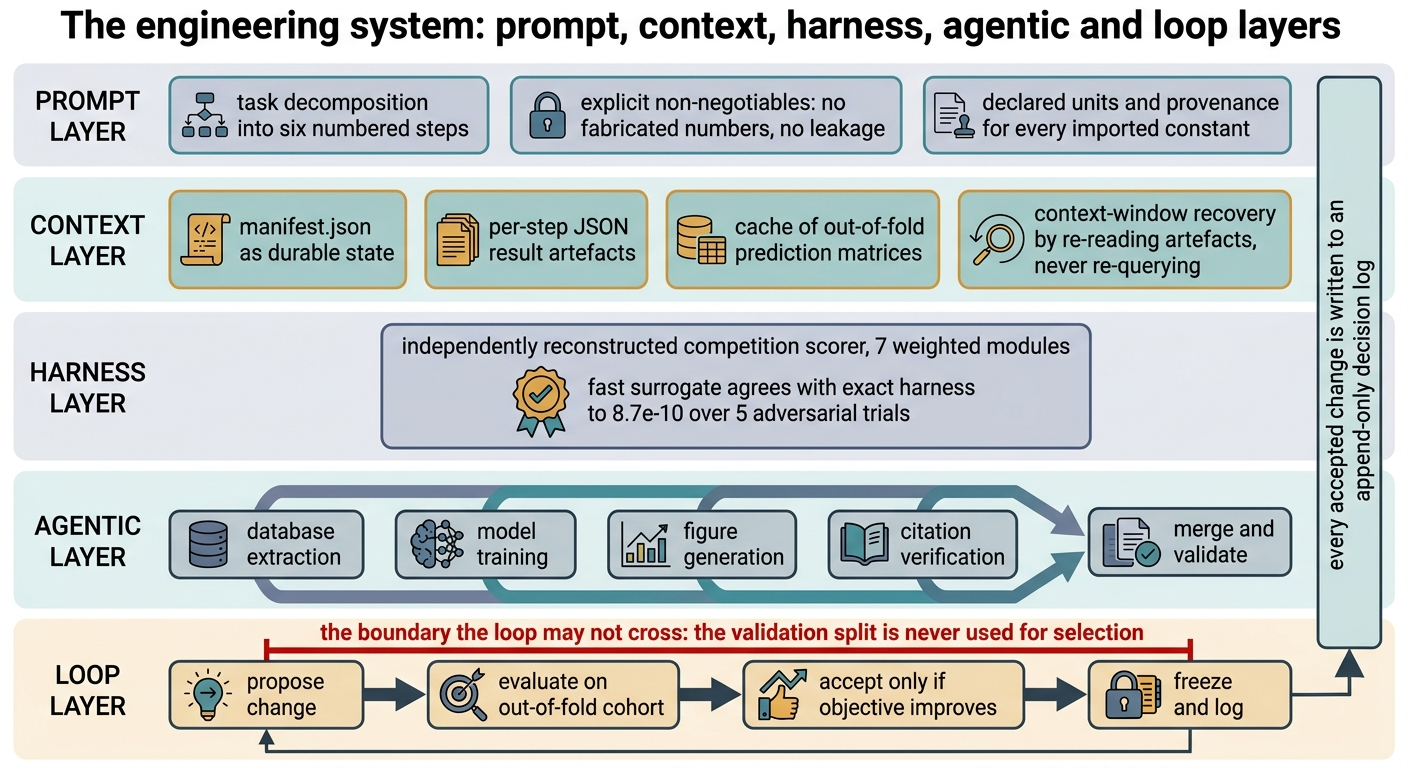
\includegraphics[width=0.94\textwidth]{figures/paper6_engineering_system.png}
\caption{\textbf{五层开发体系。} \textbf{prompt} 层固定不可协商项，其枢纽是严格区分\emph{完整性失败}（缺陷，必须抛错中止）与\emph{判据失败}（科学结果，必须如实报告并带入下一阶段）——正是这条区分使「没达到目标」成为可以写下来的结论。\textbf{context} 层以机器可读清单（\file{manifest.json}）与逐阶段产物作为跨上下文窗口的持久记忆，\emph{产物先于叙述写出}。\textbf{harness} 层是不可变的评分真值，快速代理相对它的实测偏差在 $10^{-10}$--$10^{-9}$ 量级，远优于 $10^{-6}$ 的强制门限。\textbf{agentic} 层只把\emph{有界且可校验}的任务并行化（数据库抽取、模型训练、图件生成、引用核验），被刻意排除在需要判断的环节之外——一个 DOI 可以被廉价核对，一个解释不能。\textbf{loop} 层执行「提议 $\to$ 变异 $\to$ 快速评分 $\to$ 诊断 $\to$ Pareto 保留」，红线以协议写死：变异只作用于配置，\textbf{评分代码、队列定义与折划分永不变异}。}
\label{fig:engsys}
\end{figure}

自演化环路实际运行 \textbf{12 次迭代、接受 4 次、崩溃 0 次}，在 \textbf{955.7 秒内完成 176\,393 次快速目标评估}（用精确评分器执行同样搜索约需 1\,337 机时），Pareto 前沿（折外目标 $\uparrow$，自由参数数 $\downarrow$）最终含 5 个点。需要说明其与部署配置的关系：\textbf{阶段 5 部署配置来自簇数阶梯的折外选择而非该环路}（环路最优 k16/$\alpha=0.005$ 的折外快速目标 0.461915，与部署配置的折外精确总分 0.463067 不在同一口径上，且环路日志写入时间晚于部署配置的冻结时间），故本方案把它作为\textbf{方法论组件与独立复核}报告，\emph{不宣称成绩由它取得}。环路还包含一处比原计划\textbf{更保守}的偏离：Pareto 轴由「折外目标、若晋升的验证分」改为「折外目标、自由参数数」，因为把验证分放进保留规则会使验证在迭代间变成调参信号。
